\section{The Design Space of Tubes}

\begin{figure}[h]
\centering
    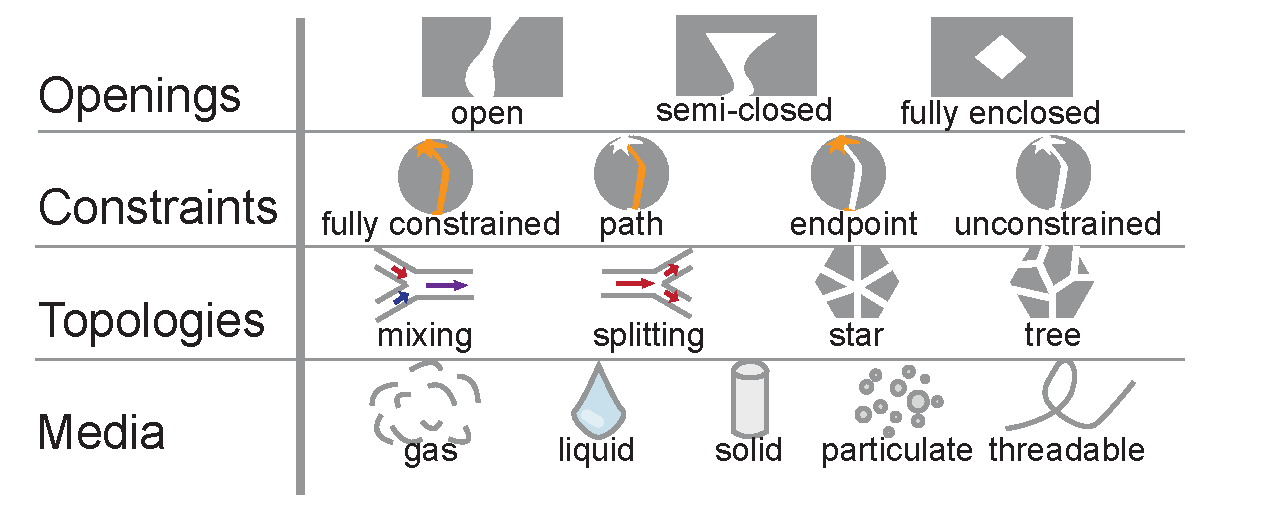
\includegraphics[width=3.4in]{figures/tubespace.png}
\caption{The design space of tubes.  Tube types, media, topologies, and design are discussed more fully in the text.}
\label{fig:tubespace}
\end{figure}

\subsection{Types of Tubes}

Tubes can come in four types: open, return, semi-closed, and fully enclosed.  Each of these types offers distinct interaction capabilities (see Figure \ref{fig:tubespace}).

Open tubes originate from the system side and connect the user side, with both ends of the tube open.  This type of tube may be used to create, for example, capacitive sensors: an open tube filled with conductive paint can be connected to a sensing platform (e.g., Arduino) on the system side, while a user can touch the uncapped other end of the tube.  Using Swept Frequency Capacitive Sensing \cite{Sato-touche} or other techniques, a user's touch of the open end can be sensed.  An open tube can also be used for output, for example by creating in-air vortices as in \cite{Sodhi-aireal}.

A return tube originates at the system and returns back to it.  By threading an electroluminescent (EL) wire through a clear return tube, a maker can create a custom piece of neon art.  If a return tube passes very close to the surface of a 3D printed model, warm or cold water passed through the tube could be used for temperature-based haptic feedback.

Semi-closed tubes are open at the system end (for control of the enclosed medium) and closed at the user end.  We believe this closed interface is most interesting when it is fabricated from a mobile material: for example, a series of tubes terminated in thin rubber membranes on the user side can be actuated by an air pump to create haptic feedback.  Without a printer capable of fabricating flexible material, a maker could affix a balloon to an open tube's end to behave similarly; another possibility is to use semi-closed tubes as audio-generating resonance chambers.

While possible to create, a tube which is open on the user side and closed on the system side is outside our focus is on computer-mediated interaction, and we therefore do not discuss these tubes.

A fully enclosed tube has no openings on either the system side or the user side.  Fully enclosed tubes can be used as resonance chambers (e.g., for object identification), or as air bubbles (e.g., as used in \cite{Willis-printedoptics} for internal display).  Their physical design space is very limited, as any support material required to create their internal geometry cannot be accessed for removal.

\subsection{Media in Tubes}

Tubes can be filled with a variety of media to create different interface affordances and capabilities.

``Gas'' comprises all compressible fluids.  Use of fluid pressure inside tubes can create haptic feedback at semi-closed interfaces, or the gases can be used as carriers for scents or fog.  As in \cite{Slyper-pressure}, structures can be engineered to change in air pressure when manipulated correctly (e.g., a spiral that changes pressure when twisted, but not pressed), and thus fluid pressure can also be used as an input.

Incompressible fluids (``liquids'') can perform many of the same interface tasks as gases.  One opportunity with liquids is to fill the interior of tubes with them and cap the ends.  In addition, one can use driable conductive fluids, such as copper paint, to coat the interior of tubes and allow them to function as arbitrarily-shaped wires.  This is especially helpful for the creation of a shared ground, or for creating single-wire capacitive interfaces amenable to sensing with SFCS \cite{Sato-touche}.

Tubes need not have hollow centers: in the case where routed tubes are filled with solid material---in particular, a solid material different from the model material---, interactions such as those in \cite{Willis-printedoptics} are possible.

Particulates, either printed in-place or inserted, can be of varying densities.  A single particle can be used for display.  Sparse particles in a stream of fluid can provide haptic feedback.  Dense particles in a semi-closed tube allow for jamming-based interactions at any point on the surface of an object \cite{Follmer-jamming}.

Threadable inserted elements, such as electroluminescent (EL) wire or fiberoptic cables, are those that can be threaded through tubes post-printing.  This allows overcoming limitations of printers: for example, a Printed Optics-style interface can be created on an inexpensive consumer-grade 3D printer using tubes and inserted fiber optic cable.

\subsection{Topological variations}

Tube topology enables different types of interactions.

Splitting or mixing tubes offer flexibility in output.  If a maker wished to create a painting device, she might wish to have two system-side tubes feeding in primary-colored red and blue paints which mix in varying ratios, allowing their pigments to combine before purple exits from the device (see Figure \ref{fig:tubespace}).  Splitting can also be useful, for example if our maker wants red paint output in two locations from her painting device, she could have one system-side tube, but split the tube into two (see Figure \ref{fig:tubespace}).

Star and tree topologies are extensions of the splitting and mixing primitives.  Using a star topology in which the tubes were filled with conductive paint, we created a toy with several touch-sensitive areas, see Figure \ref{fig:toy}.

\subsection{Features of Tubes}

Tubes may emphasize either their exterior features (connection points) or their interior paths.  These two features lead to different kinds of interfaces.  An example interface that focuses on the exterior connection points is the touch sensitive toy in Figure \ref{fig:toy}, where tubes must exit the toy at the eyes, ears, tail, etc.  An interface focused on the internal path of the tube is the neon sign in Figure \ref{fig:neon}: output is based on the shape of the tube.

\subsection{Inputs and Outputs}

\valkyrie{we can just include related work in this section?  we basically cover it in the table, anyway.}

\begin{figure*}[t]
\centering
    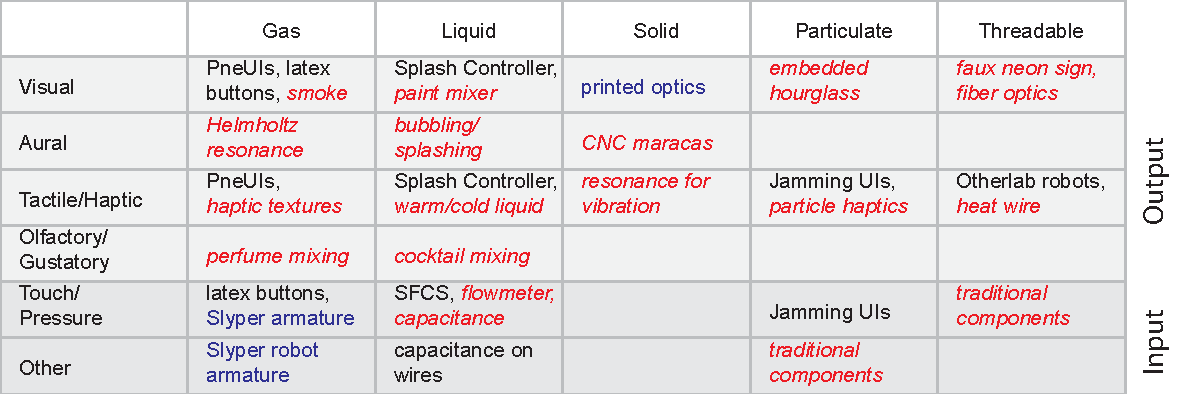
\includegraphics[width=\textwidth]{figures/designspace.png}
\caption{The design space of tube-based interactions.  Existing systems are written in regular font.  Those created with fabrication are in {\color{blue}blue}. In \emph{{\color{red}red italic}} are unexplored interactions creatable with custom-fabricated tubes.  Darker grey is output.  Lighter grey is input.  \valkyrie{I don't know what else might go in the blank spaces... looking for suggestions!  Also, I'm not confident this breakdown is the most clear: for example, the "liquids" category includes the copper paint, which functions as wires ("threadables"), but takes the form of a liquid...}}
\label{fig-designspace}
\end{figure*}

\valkyrie{optimally, we can just describe this thoroughly in the chart, and avoid spending a bazillion paragraphs talking about each thing individually here}

\subsection{Inputs}

\subsubsection{Flexing}

Much like \cite{Slyper-shape}, we can sense flexing and bending of prints made on the Objet.  We can make prints on the Objet and tunnel through them, though, without making crazytastic silicone molds.  We can make things flex using muscle wire and cleverly-placed expandable air pockets.

\subsubsection{Touch}
Capacitance (digital).  SFCS.

\subsubsection{Pressure}
Pressure (via SFCS or fluid pressure). 

\subsubsection{Tapping}
 Tapping (audio/resonance?) carried through particular tubes, like we talked about hard tubes in a soft thing.  We use hard tubes in soft things, anyway, for the conductive goo.

\subsubsection{Other stuff?}
Could be.

\subsubsection{Traditional Components}
Obviously you can hook up traditional buttons, etc., the same way as always.  With copper paint instead of traditional wiring, we can share grounds, and we don't have to solder.

\subsection{Outputs}

\subsubsection{Visual}
EL wire.  Colored liquids.  Mechanical motion by pushing light or tube-plugging (like a big ball) objects with fluid.

\subsubsection{Aural}
Resonance chambers.  Air cavity design for sound/amplification (see passive iPhone speakers).  I mean, this is basically just 3D printing instruments, which we know has been done.

\subsubsection{Haptic}
Compressible and incompressible fluids for actuation.  Recreation of PneUIs.  Tactile output.  Adding particles to add extra feedback.

\subsubsection{Olfactory/Gustatory}
Different chambers filled with different scented/flavored fluids.  We can mix them using pipes and pressure.

\subsection{Identity}

Tubes included in printed objects allow for their identification.  While the tubes need not be visible (especially in the case of fully-enclosed tubes), their presence, location, and length change the acoustic resonance properties of a printed object.

Both identification by recall and intentional encoding are possible.  As seen in \cite{Ono-touchandactivate}, different objects have different acoustic signatures.  The presence of tubes changes this, thus allowing for recall of a shape once its acoustic signature has been recorded.  In addition, semi-closed tubes can function as resonance chambers: the first resonant frequency $F_1$ Hz of a semi-closed tube length $L$ meters can be found by $F_1 = \frac{c}{4L}$ (where $c$ is the speed of sound).  All odd harmonics (i.e., $3*F_1$, $5*F_1$, $7*F_1$, ...) of this frequency are also resonant frequencies of the tube.

An object's resonant frequency can be measured by attaching a speaker and microphone to it, sweeping frequencies with the speaker, and performing a Fourier transform on the resultant signal from the microphone.  Peaks in the transformed data correspond to stronger returned impulses: the resonant frequencies of the object.  

\valkyrie{in my experiments so far, it seems that the material printed does conduct sound fairly well, so this is feasible.  I think we should get some equipment and do a small test, though, since I don't know how the resonance will change with the big hunk of plastic around the semi-open tube.  hopefully discussing this with Alex soon.}